\documentclass{standalone}
\usepackage{tikz}
\usepackage{ctex,siunitx}
\usepackage{tkz-euclide}
\usepackage{amsmath}
\usetikzlibrary{patterns, calc}
\usetikzlibrary {decorations.pathmorphing, decorations.pathreplacing, decorations.shapes,}
\begin{document}
\small
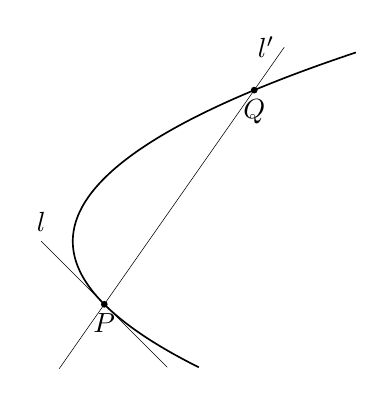
\begin{tikzpicture}[>=latex,scale=0.8]
  \tkzDefPoints{0.5/-1/P,0/-0.5/Pl,2.88/2.4/Q}
  \draw[semithick,domain=-2:3,samples=200] plot({0.5*\x*\x},{\x});
  \tkzDrawPoints[fill=black](P,Q)
  \tkzDrawLine[add = 2 and 1](P,Pl)
  \tkzLabelLine[pos=2.0,above](P,Pl){$l$}
  \tkzDrawLine[add = 0.3 and 0.2](P,Q)
  \tkzLabelLine[pos=1.2,left](P,Q){$l'$}
  \tkzLabelPoints[below](P,Q)
\end{tikzpicture}
\end{document}